The following data was used from Kaviar for research:

\begin{itemize}
\item CG variants
\item 90K unverified SNVs
\item 54K unverified indels
\item Verified variants (CG and Illumina)
\item 170K verified SNVs
\item 4K verified indels

\item Regional features associated with sequencing problems:
\item Repeat-masker
\item Blacklist regions
\item CG content
\item Mappability

\end{itemize}

Details and steps taken with variant preparation:

\begin{itemize}
\item Downsampled dominant classes to have equally sized datasets
\item 50 percent of CG unverified indels were at least 10bp away from Illumina indels
\end{itemize}

\begin{alertblock}{Important Result}

Lorem ipsum dolor \textbf{sit amet}, consectetur adipiscing elit. Sed commodo molestie porta. Sed ultrices scelerisque sapien ac commodo. Donec ut volutpat elit.

\end{alertblock} 

\begin{figure}
\includegraphics[width=0.9\linewidth]{placeholder.jpg}
\caption{Workflow}
\end{figure}

\begin{block}{Results}

\begin{figure}
\includegraphics[width=0.8\linewidth]{placeholder.jpg}
\caption{Figure caption}
\end{figure}

Performance of random forest for indel variants had accuracy of 75 percent.
Performance of random forest for SNV variants had accuracy of 58 percent.
Performance of random forest on all variant types led to an accuracy of 62 percent.
:

\begin{table}
\vspace{2ex}
\begin{tabular}{l l l}
\toprule
\textbf{Treatments} & \textbf{Response 1} & \textbf{Response 2}\\
\midrule
Treatment 1 & 0.0003262 & 0.562 \\
Treatment 2 & 0.0015681 & 0.910 \\
Treatment 3 & 0.0009271 & 0.296 \\
\bottomrule
\end{tabular}
\caption{Table caption}
\end{table}

\end{block}

\begin{alertblock}{Contact Information}

\begin{itemize}
\item Email: \href{mailto:john@smith.com}{evansj@email.chop.edu}
\end{itemize}

\end{alertblock}
\begin{block}{Acknowledgements}

\small{\rmfamily{Nam mollis tristique neque eu luctus. Suspendisse rutrum congue nisi sed convallis. Aenean id neque dolor. Pellentesque habitant morbi tristique senectus et netus et malesuada fames ac turpis egestas.}} \\

\end{block}

%----------------------------------------------------------------------------------------
%	CONTACT INFORMATION
%----------------------------------------------------------------------------------------



\begin{center}
\begin{tabular}{ccc}
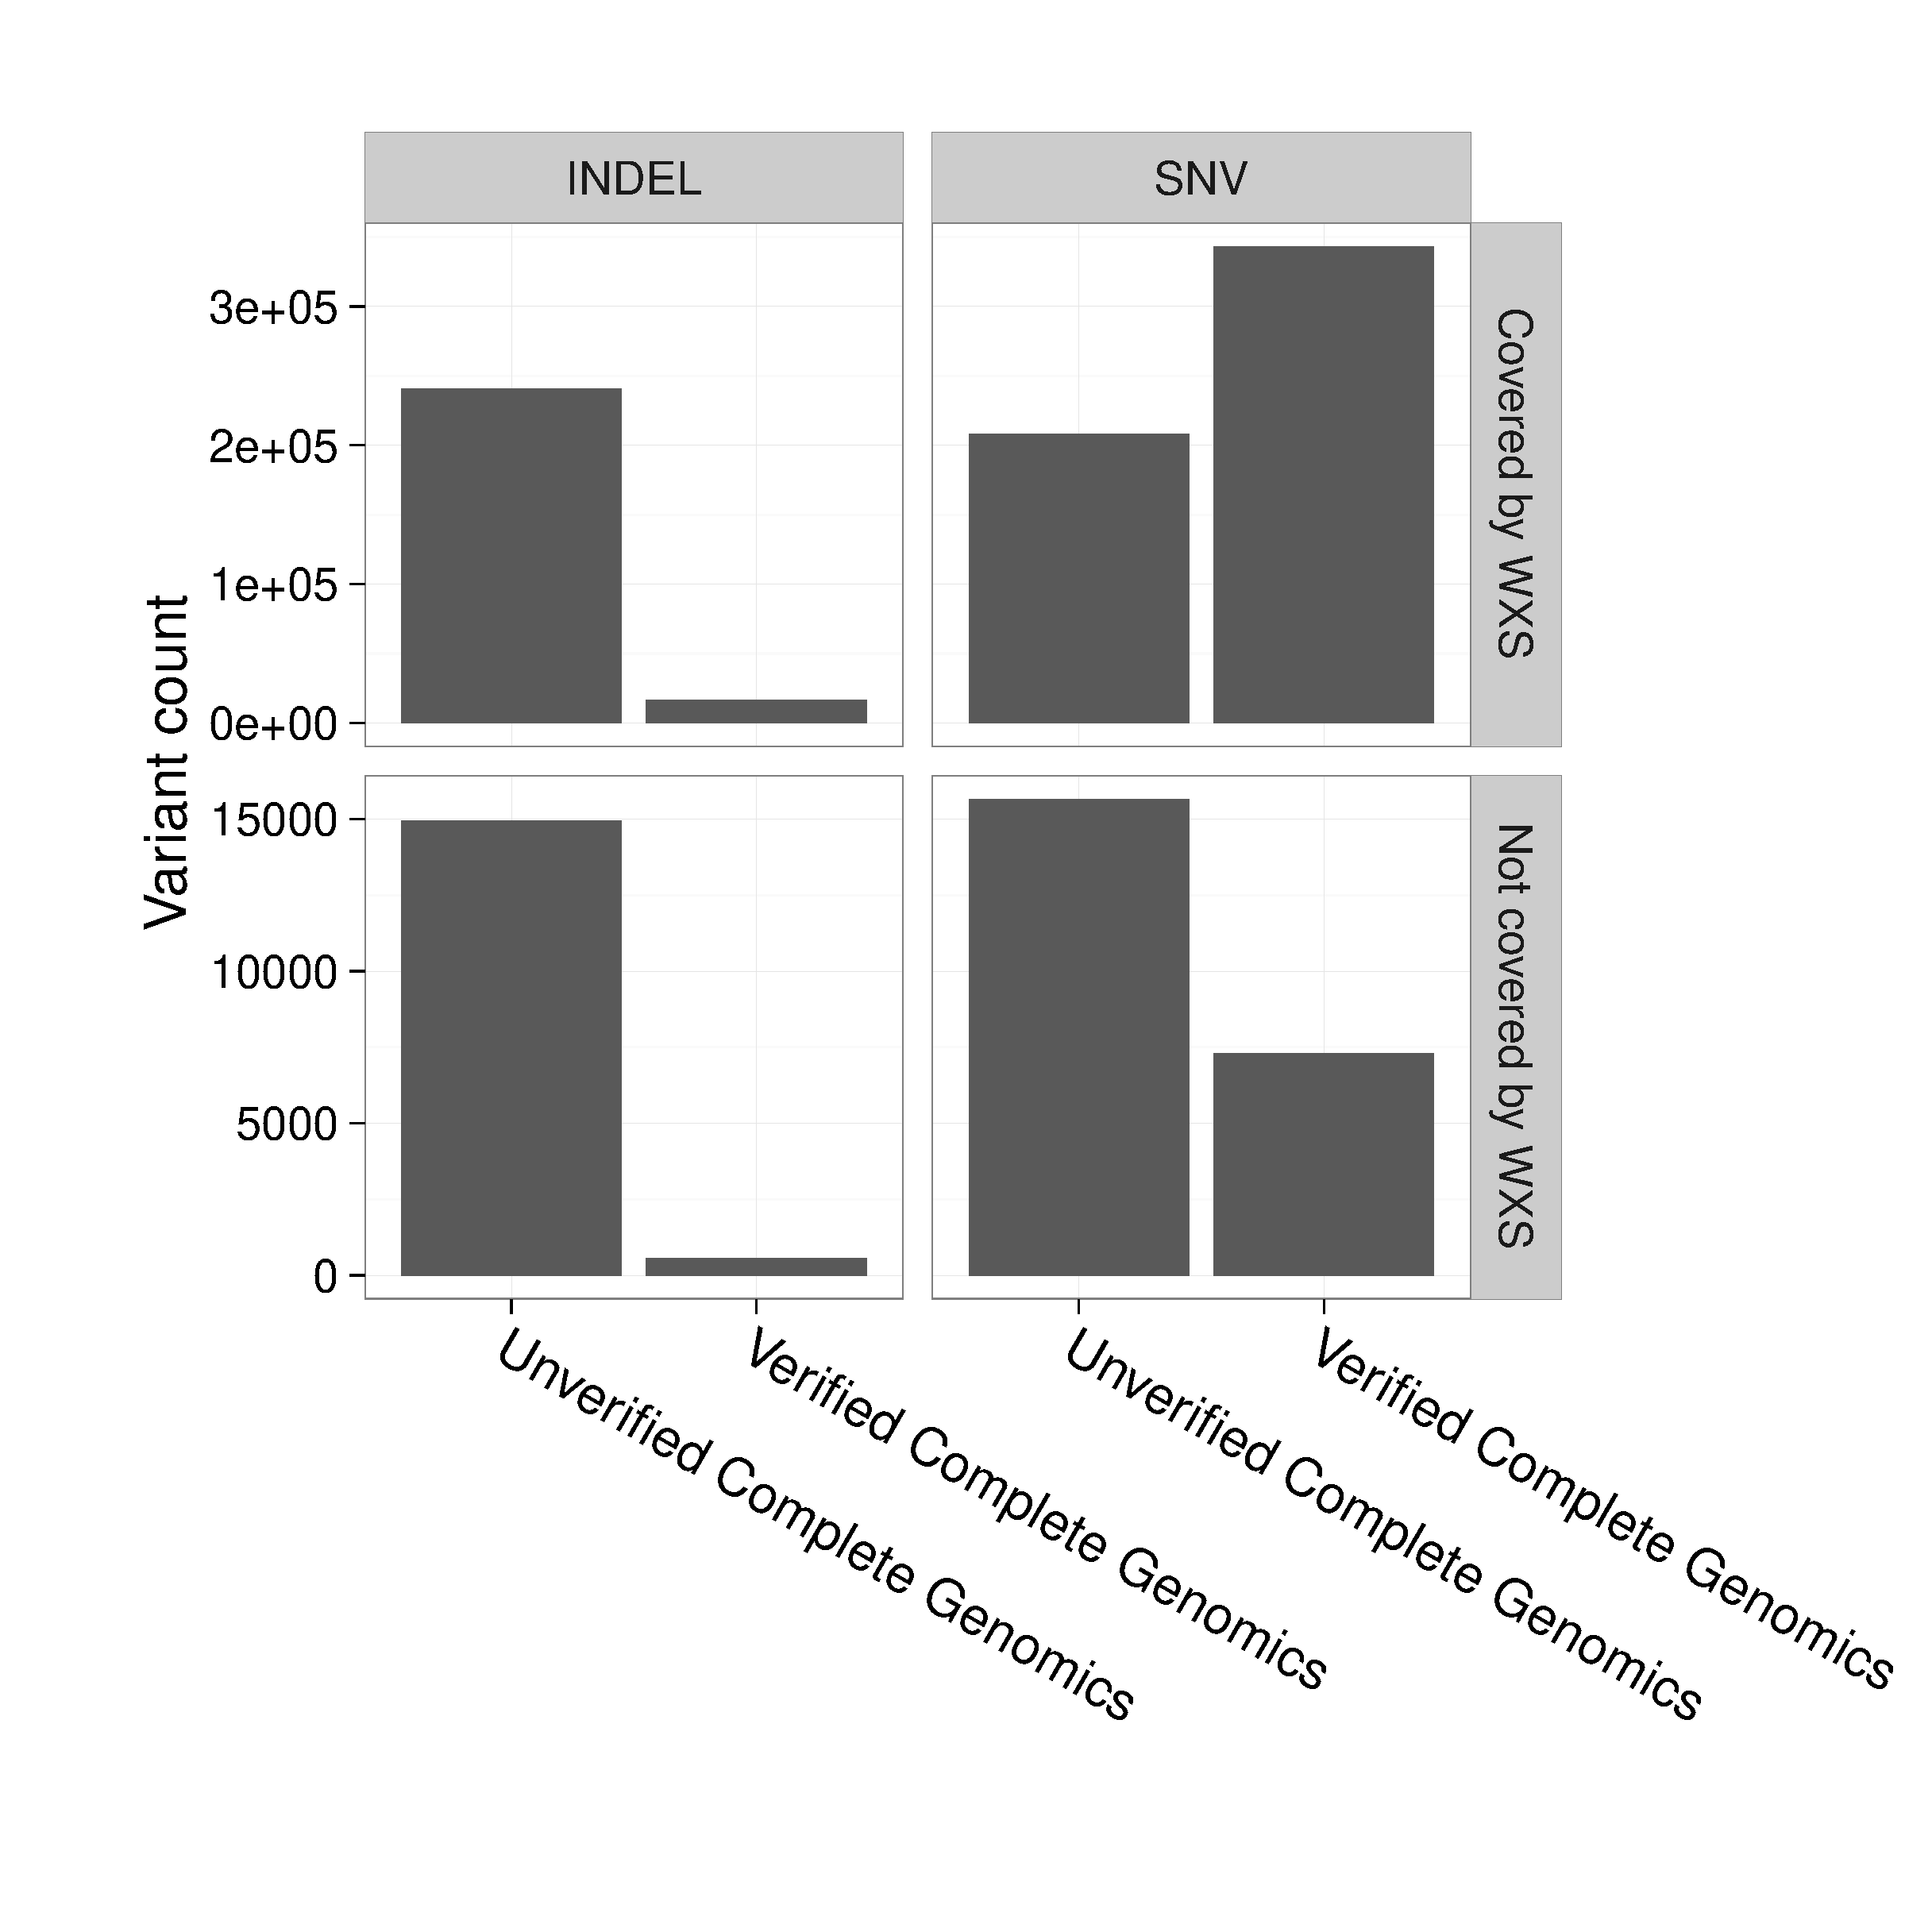
\includegraphics[width=0.5\linewidth]{init_counts.eps} & \hfill & 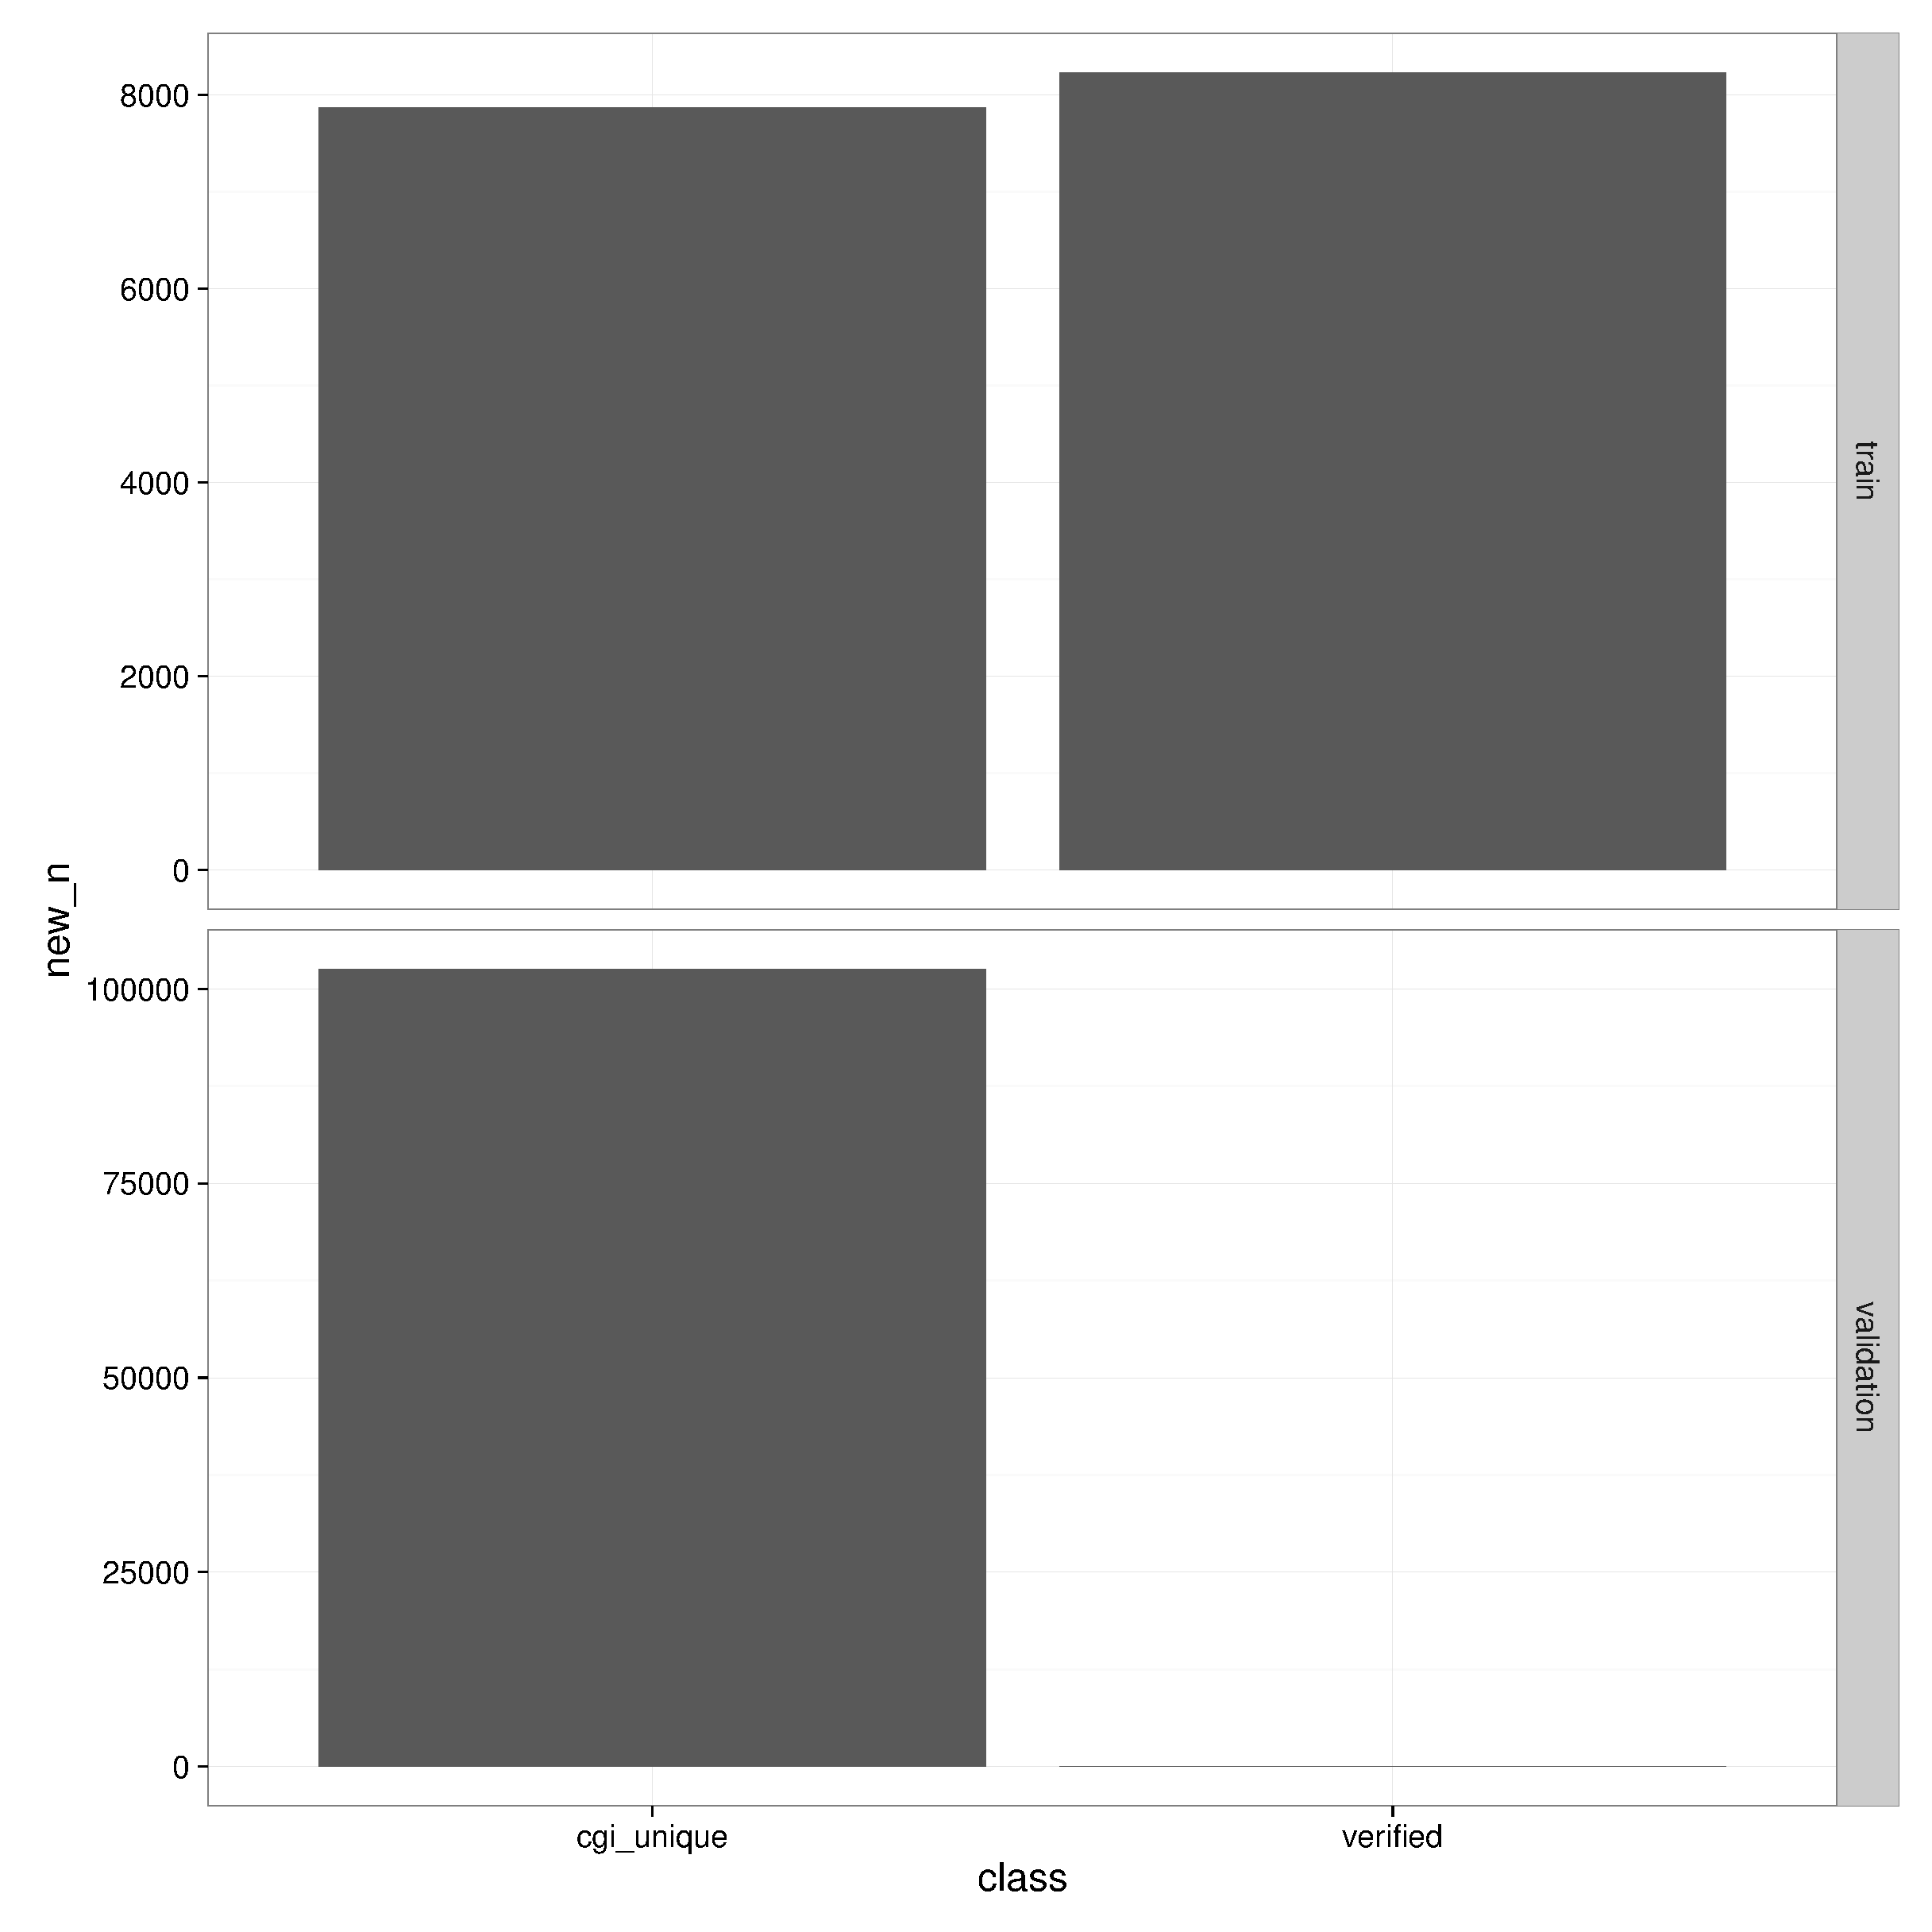
\includegraphics[width=0.5\linewidth]{counts.eps}
\end{tabular}
\end{center}

\begin{alertblock}{Objectives}

Variant calls by different sequencing platform need to be analyzed differently and are throughout many different databases:
\begin{itemize}
\item Can CG and Illumina variants be split by position features?
\item Use Kaviar data set to build a classifier to determine sequencing platform source for variants.
\item Provide results from classifier to assist with filtering variant calls  
\end{itemize}

\end{alertblock}

Upon filtering and flanking indel calls, the reference sequences corresponding to these indels were annotated for the insertion or deletion and a indel representation sequence was made. The data was sampled and entered into the network for training which performed and additional sampling of this input.